\section{Extensions}
\label{kvdirect:sec:extensions}

\subsection{基于 CPU 的分散 - 聚集 DMA}


对于64B DMA操作,PCIe具有29%的TLP报头和填充开销(\ S \ ref {kvdirect:sec:challenge}),并且DMA引擎可能没有足够的并行性来使用小TLP(\ S)使PCIe带宽延迟产品饱和\ REF{kvdirect:秒:实施})。
我们系统中的PCIe根联合体支持更大的DMA操作,最高256字节的TLP有效负载。 在这种情况下,TLP头和填充开销仅为9%,并且DMA引擎具有足够的并行性(64)以通过27个正在进行的DMA读取来使PCIe链路饱和。
要批量处理PCIe链路上的DMA操作,我们可以利用CPU来执行分散 - 聚集(scatter gather)(图〜\ ref {kvdirect:fig:sg-arch})。
首先,NIC DMA将地址发送到主机内存中的请求队列。 主机CPU轮询请求队列,执行随机内存访问,将数据放入响应队列并将MMIO门铃写入NIC。 然后,NIC通过DMA从响应队列中提取数据。

\begin{figure}[t]
\centering
\subfloat[Read.\label{kvdirect:fig:sge-read}]
{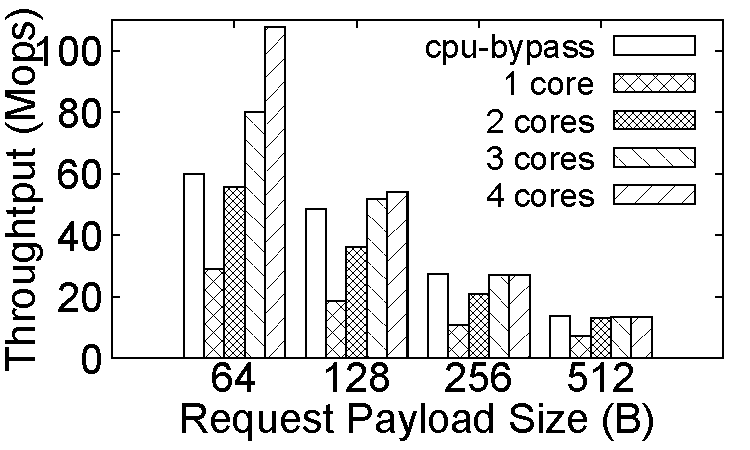
\includegraphics[width=.5\textwidth,page=1]{sg-read.pdf}}
\subfloat[Write.\label{kvdirect:fig:sge-write}]
{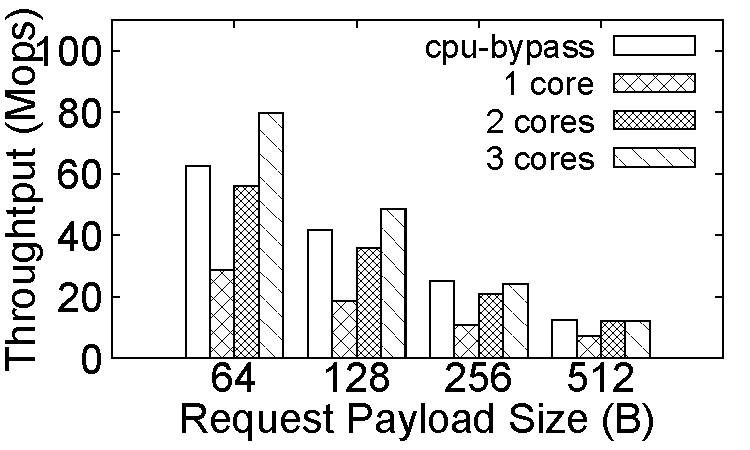
\includegraphics[width=.5\textwidth,page=1]{sg-write.pdf}}
\caption{Scatter-gather performance.}
\label{kvdirect:fig:scatter-gather}

\end{figure}

图 \ref {kvdirect:fig:scatter-gather} 表明,与CPU旁路方法相比,基于CPU的分散 - 聚集DMA的吞吐量提高了79%。
除了CPU开销之外,基于CPU的分散 - 聚集的主要缺点是额外的延迟。
为了将MMIO从CPU保存到NIC,我们每个门铃批量256个DMA操作,这需要 10 $\mu$s 才能完成。
使用基于CPU的分散 - 聚集NIC访问主机内存的总延迟是大约20美元,比直接DMA高出近20倍。

\subsection{单机多网卡}
\label{kvdirect:sec:multi-nic}

\begin{figure}[t]
\begin{minipage}[t]{0.5\textwidth}
\centering
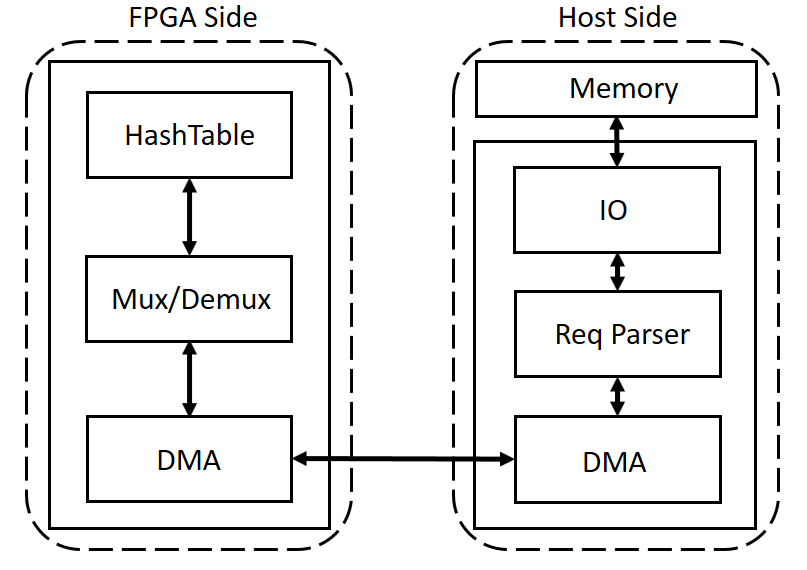
\includegraphics[width=1\textwidth,page=1]{scatter_gather.PNG}
\caption{分散 - 聚集(scatter-gather)架构。}
\label{kvdirect:fig:sg-arch}
\end{minipage}
\begin{minipage}[t]{0.5\textwidth}
\centering
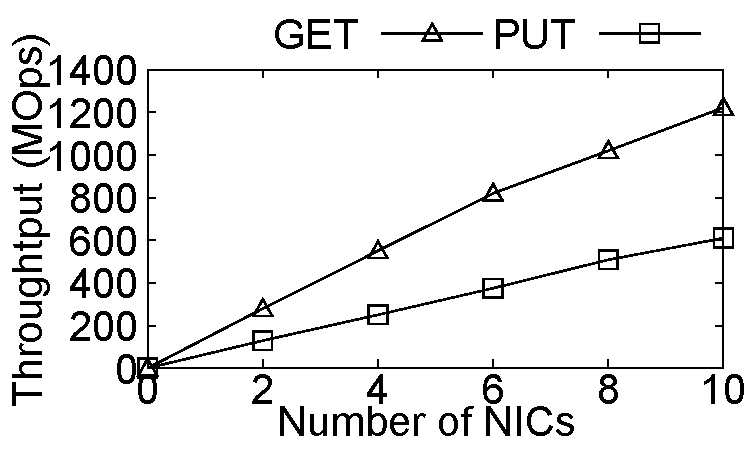
\includegraphics[width=1\textwidth,page=1]{multi_nic.pdf}
\caption{单机多网卡的性能可扩放性。}
\label{kvdirect:fig:multiple-nics}
\end{minipage}

\end{figure}

KV-Direct的主要用例是启用远程直接键值访问,而无需服务器上的CPU开销。
在某些情况下,可能需要构建一个具有每服务器最大吞吐量的专用键值存储。
通过模拟,\cite {li2016full}显示了在具有四个(当前不可用的)60核CPU的单个服务器中实现十亿KV运行的可能性。
如表 \ref{kvdirect:tab:kvs-compare}所示,在服务器上有10个KV-Direct NIC,使用商用服务器可以轻松实现10亿KV op / s性能。
服务器消耗357瓦的功率(在墙壁上测量)以达到1.22~Gop / s GET或0.61~Gop / s PUT。

为了使两个Xeon E5 CPU的80个PCIe Gen3通道饱和,我们用带有10个PCIe Gen3 x8插槽的 SuperMicro X9DRX+-F 主板替换了基准测试服务器的主板(\S\ref {kvdirect:sec:eval}) 。
我们使用PCIe x16到x8转换器连接每个插槽上的10个可编程网卡,每个网卡上只启用一个PCIe Gen3 x8链路,因此每个网卡的吞吐量低于图 \ref {kvdirect:fig:ycsb-tput}。
每个NIC在主机内存中拥有一个独占内存区域,并提供不相交的密钥分区。
多个NIC遇到与多核KVS实现相同的负载不平衡问题。
幸运的是,对于少量分区(\textit {例如10个}),负载不平衡并不重要 \cite {lim2014mica,li2016full}。在YCSB长尾工作负载下,负载最高的NIC的平均负载为1.5倍,非常流行的密钥所增加的负载由无序执行引擎提供(\S \ref {kvdirect:sec:ooo})。
相比之下,为了实现与240个CPU内核的匹配性能,最热芯的负载将是平均值的10倍。
图\ref {kvdirect:fig:multiple-nics}显示KV-Direct吞吐量几乎与服务器上的NIC数量呈线性关系。

\subsection{访问 SSD}

\textbf{TODO}


\subsection{有状态网络功能的存储}

\textbf{TODO,网卡大量并发连接……}


\section{讨论}
\label{kvdirect:sec:discussion}

\subsection{不同容量的网卡硬件}
\label{kvdirect:sec:different-nic}

KV-Direct的目标是利用数据中心的现有硬件来卸载重要的工作负载(KV访问),而不是设计特殊的硬件来实现最大的KVS性能。 我们使用可编程NIC,它通常包含有限数量的DRAM用于缓冲和连接状态跟踪。 大型DRAM在芯片尺寸和功耗方面都很昂贵。

\begin{table}[t]
\centering
\scalebox{0.85}{
\begin{tabular}{|l|r|r|r|r|r|r|}
\hline
     & 1/1024 & 1/256 & 1/64 & 1/16 & 1/4 & 1 \\
\hline
1/2  & 0.366 & 0.358 & 0.350 & 0.342 & 0.335 & 0.327 \\
\hline
1    & 0.583 & 0.562 & 0.543 & 0.525 & 0.508 & 0.492 \\
\hline
2    & 0.830 & 0.789 & 0.752 & 0.718 & 0.687 & 0.658 \\
\hline
4    & 1     & 0.991 & 0.933 & 0.881 & 0.835 & 0.793 \\
\hline
8    & 1     & 1     & 1     & 0.995 & 0.937 & 0.885 \\
\hline
\end{tabular}
}
\caption{不同NIC DRAM / PCIe吞吐率(垂直)和NIC /主机内存大小比(水平)下长尾工作负载的最佳负载分配比。}
\label{kvdirect:tab:optimal-load-dispatch}

\end{table}

\begin{table}[t]
\centering
\scalebox{0.85}{
\begin{tabular}{|l|r|r|r|r|r|r|}
\hline
    & 1/1024 & 1/256 & 1/64 & 1/16 & 1/4 & 1 \\
\hline
1/2 & 1.36	& 1.39	& 1.40	& 1.37	& 1.19	& 1.02 \\ 
\hline
1	& 1.71	& 1.77	& 1.81	& 1.79	& 1.57	& 1.01 \\
\hline
2	& 2.40	& 2.52	& 2.62	& 2.62	& 2.33	& 1.52 \\
\hline
4	& 3.99	& 4.02	& 4.22	& 4.27	& 3.83	& 2.52 \\
\hline
8	& 7.99	& 7.97	& 7.87	& 7.56	& 6.83	& 4.52 \\
\hline
\end{tabular}
}
\caption{与简单分区相比,负载分派的相对吞吐量。 列标题与表格相同~\ref{kvdirect:tab:optimal-load-dispatch}。}
\label{kvdirect:tab:optimal-load-dispatch-throughput}

\end{table}


即使未来的NIC具有更快或更大的板载内存,在长尾工作负载下,我们的负载分配设计(\S \ref {kvdirect:sec:dram-cache})仍然显示出比简单的分区设计更高的性能。密钥统一根据NIC和主机内存容量。
表 \ref {kvdirect:tab:optimal-load-dispatch} 显示了具有10亿个密钥的长尾工作负载的最佳负载分配比率,不同的NIC DRAM和PCIe吞吐率以及不同的NIC和主机比率内存大小。
如果NIC具有更快的DRAM,则将更多负载分派给NIC。负载分配比率为1表示NIC内存的行为与主机内存的高速缓存完全相同。
如果NIC具有更大的DRAM,则将稍微少量的负载分派给NIC。
如表 \ref {kvdirect:tab:optimal-load-dispatch-throughput} 所示,即使NIC DRAM的大小只是主机内存的一小部分,吞吐量增益也很大。

乱序执行引擎(\S \ref {kvdirect:sec:ooo})可以应用于需要隐藏延迟的各种应用程序,我们希望未来的RDMA NIC能够支持原子的。

在40~Gbps网络中,网络带宽限制了非批量KV吞吐量,因此我们使用客户端批处理(\S \ref {kvdirect:sec:implementation})。通过更高的网络带宽,可以减少批量大小,从而减少延迟。在200~Gbps网络中,KV-Direct网卡无需批量即可达到180~Mop / s。

KV-Direct利用广泛部署的可编程NIC和FPGA实现 \cite{putnam2014reconfigurable,caulfield2016cloud}。 FlexNIC \cite {kaufmann2015flexnic,kaufmann2016krishnamurthy} 是另一种具有可重构匹配行动表(RMT) \cite {bosshart2013forwarding} 的可编程NIC的有前途的架构。
NetCache \cite {netcache-sosp17} 在基于RMT的可编程交换机中实现KV缓存,显示了在基于RMT的NIC中构建KV-Direct的潜力。

\subsection{对现实世界应用的影响}

当KV-Direct应用于端到端应用程序时,后台计算显示了潜在的性能提升。 在PageRank \cite {page1999pagerank}中,由于每次边缘遍历都可以通过一次KV操作实现,因此KV-Direct在具有10个可编程NIC的服务器上支持1.22G TEPS。 相比之下,GRAM \cite {wu2015g}支持每台服务器250M TEPS,受交错计算和随机内存访问的约束。

KV-Direct支持用户定义的函数和向量操作(表 \ref {kvdirect:tab:kv-operations}),可以通过将客户端计算卸载到硬件来进一步优化PageRank。 类似的参数适用于参数server \cite {li2014scaling}。 我们希望未来的工作可以利用硬件加速的键值存储来提高分布式应用程序的性能。

\subsection{键值映射以外的其他数据结构}

\textbf{TODO}